\documentclass[slidetop,12pt]{beamer}
\usepackage[T1]{fontenc}
\usepackage[latin1]{inputenc}
\usepackage[frenchb]{babel}
% pour un pdf lisible � l'�cran si on ne dispose pas
% des fontes cmsuper ou lmodern
%\usepackage{lmodern}
\usepackage{aeguill}
%\hypersetup{pdfpagemode=FullScreen}

% ------------------------------------------------
%-----------   styles pour beamer   --------------
% ------------------------------------------------
\definecolor{fondtitre}{HTML}{336E17}
\definecolor{coultitre}{RGB}{105,13,13}
\xdefinecolor{fondtexte}{rgb}{1,0.95,0.86}     % ivoire
% -------------- Fioritures de style -------------
\beamertemplatetransparentcovered
% Mettre les icones de navigation en mode vertical (pour projection)
%\setbeamertemplate{navigation symbols}[vertical]
% ------------ Choix des th�mes ------------------
\usecolortheme{crane}
\setbeamercolor{bas}{fg=coultitre, bg=fondtitre!40}
\setbeamercolor{haut}{fg=fondtitre!40, bg=coultitre}
\beamerboxesdeclarecolorscheme{clair}{fondtitre!70}{coultitre!20}
\beamerboxesdeclarecolorscheme{compar}{coultitre!70}{fondtitre!20}
% ins�rer le nombre de pages
\logo{\insertframenumber/\inserttotalframenumber}
%------------ fin style beamer -------------------

% ----------- Contenu de la page de titre --------
\title{Grid in a Grid}
\subtitle{Deployment of a gLite Grid inside Grid'5000}
\author{S�bastien Badia -- Lucas Nussbaum }
\institute{LORIA - INRIA Nancy -- Grand-Est}
\date{Grid'5000 Spring School -- April 2011}
% ------------------------------------------------

% enlarge your beamer
\setbeamersize{text margin left=3mm,text margin right=3mm}
\begin{document}
\frame{\titlepage}
%------------------ Sommaire ---------------
% 1 Intro
% 2 gLite Midelware
% 3 Demo
% 4 Next steps \LaTeX{}
\begin{frame}{Table of contents}
	\tableofcontents%[hideallsubsections]
\end{frame}

\section{Introduction}
\subsection{gLite}
\begin{frame}
\frametitle{Introduction}
	\begin{block}{gLite}
		\begin{itemize}
			\item Middleware stack for Grid Computing
			\item Developed and used by the EGI production grid\\
				{\small e.g for CERN LHC experiments\\
				330 sites, 200000 CPUs}
			\item Provides a complete \& complex set of services  for production grids
		\end{itemize}
	\end{block}
	\begin{center}
	
\includegraphics[height=1.8cm]{img/glite.png}~~~ 
	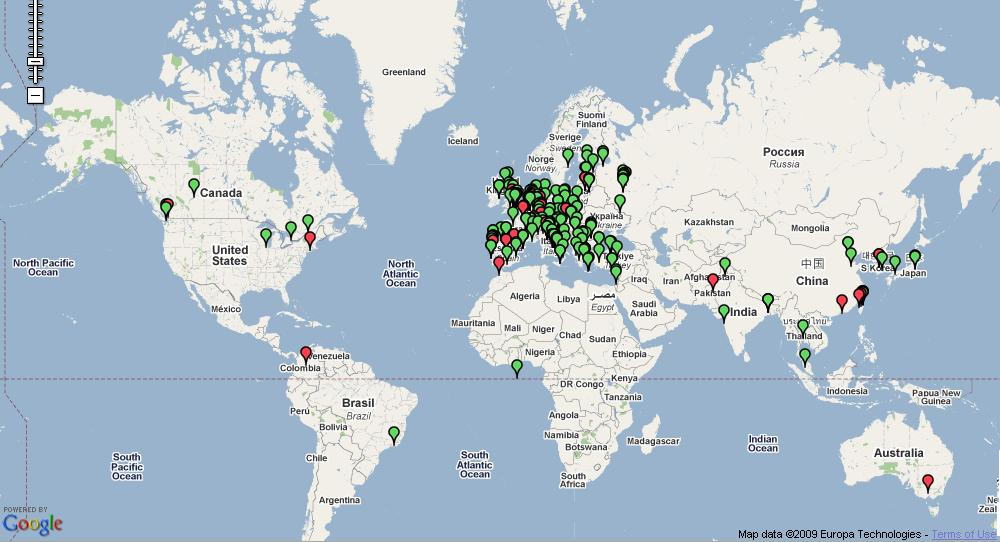
\includegraphics[height=2.4cm]{GRIDmap.jpg}~~~ 
	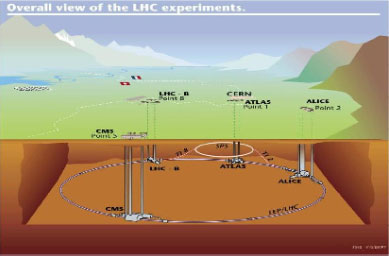
\includegraphics[height=2.4cm]{lhc.jpg}~~~ 
	\end{center}
\end{frame}
\begin{frame}{Introduction}
	\begin{block}{Improving and testing gLite}
		\begin{itemize}

			\item Difficult to improve:
				\begin{itemize}
					\item No large scale test infrastructure
					\item Cannot test on real infrastructure\\{\small risk of breaking it, low reproductibility, waste of resources}
				\end{itemize}
		\end{itemize}
		Goal of this challenge: deploy the gLite middleware on Grid'5000
		\begin{itemize}
		\item First step towards experiments on the middleware itself
		\end{itemize}
	\end{block}
	\begin{center}
	\end{center}
\end{frame}

\subsection{Scientific Linux}
\begin{frame}
\frametitle{Introduction}
	\begin{block}{Scientific Linux}
		\begin{itemize}
			\item Based on RedHat Enterprise Linux (RHEL)
			\item Version used in that experiment: Scientific Linux 5.5 (Boron)
			\item Kadeploy3 used for deployment on Grid'5000
		\end{itemize}
	\end{block}
	\begin{center}
	  
\includegraphics[width=8cm]{img/sl.jpg}
	\end{center}
\end{frame}

\subsection{gDeploy Script}
\begin{frame}
\frametitle{Introduction: gDeploy Script}
	\begin{block}{Goal}
		\begin{itemize}
			\item Deploy a gLite site
			\item composed of :
			\begin{itemize}
				\item a BDII element
			  \item a Batch scheduler
			  \item a Computing element
			  \item Workers nodes
			\end{itemize}
		\end{itemize}
	\end{block}
	\begin{block}{Script}
	  \begin{itemize}
		  \item Written in ruby, leverages the G5K API and \textsl{net-ssh-multi}
			\item available on \url{http://sbadia.github.com/gdeploy/}
		\end{itemize}
	\end{block}
\end{frame}

\section{gLite Middleware}
\subsection{Information Service}
\begin{frame}
\frametitle{gLite Middleware}
  \begin{block}{Information Service -- gLite BDII}
	\begin{itemize}
		\item Information Service is a BDII (Berkley Database Information Index), OpenLDAP Server
		\item BDII provide information about the grid ressources and their status
	\end{itemize}
	\end{block}
	\begin{center}
          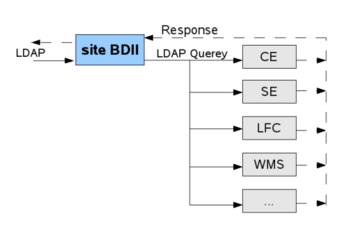
\includegraphics[width=6cm]{img/bdii.png}
        \end{center}
\end{frame}

\subsection{Batch}
\begin{frame}
\frametitle{gLite Middleware}
  \begin{block}{gLite Batch}
	\begin{itemize}
		\item Batch scheduler
		\item Queue manager
   	\end{itemize}
		\begin{beamerboxesrounded}[scheme=clair]{}
		 = Torque server + Maui scheduler
		\end{beamerboxesrounded}
	\end{block}
	\begin{center}
		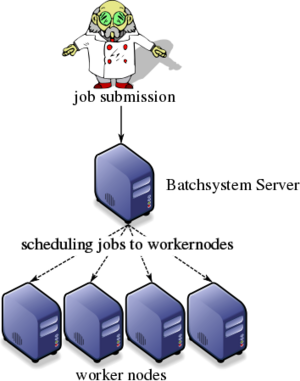
\includegraphics[width=3.5cm]{img/batch.png}
	\end{center}
\end{frame}

\subsection{Computing Element}
\begin{frame}
\frametitle{gLite Middleware}
  \begin{block}{Computing Element}
	\begin{itemize}
		\item Store information about workers nodes
		\item Interface with cluster (WN)
	\end{itemize}
		\begin{beamerboxesrounded}[scheme=clair]{}
	    Cream computing element (torque client, mysql, tomcat)
		\end{beamerboxesrounded}
	\end{block}
        \begin{center}
                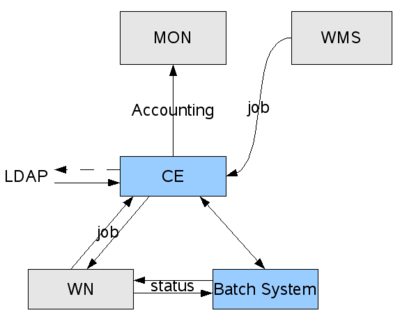
\includegraphics[width=4.5cm]{img/ce.png}
        \end{center}
\end{frame}

\subsection{Workers Nodes}
\begin{frame}
\frametitle{gLite Middleware}
  \begin{block}{Worker nodes}
	\begin{itemize}
		\item Cluster on Scientific Linux 5.5
		\item Belong to a Virtual Organisation
	\end{itemize}
	\end{block}
	\begin{center}
	  
\includegraphics[width=3cm]{img/wn.jpg}
	\end{center}
\end{frame}

\section{Demo}
\subsection{Deploy Scientific Linux}
\begin{frame}
\frametitle{Demo}
	\begin{exampleblock}{Demo}
	  \begin{itemize}
	    \item Reserve nodes and deploy Scientific Linux (using Grid'5000 API)
	    \item Launch gdeploy script
	    \item Test your gLite site
	  \end{itemize}
	\end{exampleblock}
\end{frame}

\section{Conclusion}
\subsection{Next Steps}
\begin{frame}
\frametitle{Conclusion}
\framesubtitle{Next steps}
Future work for gLite on Grid'5000
	\begin{alertblock}{TODO}
		\begin{itemize}
    	\item Generic SL image that works on all clusters
			\item Storage: SE, LFC
			 \item WMS and UI
			\item Multi-VO, inter-VO communications
		\end{itemize}
  \end{alertblock}
\end{frame}

\subsection{Sources}
\begin{frame}
\frametitle{Sources}
  \begin{block}{Sources - Links}
    \begin{itemize}
      \item \url{http://glite.web.cern.ch/glite/}
      \item \url{http://en.wikipedia.org/wiki/GLite}
      \item \url{http://www.sysadmin.hep.ac.uk/}
    \end{itemize}
  \end{block}
\end{frame}

\frame{\titlepage}
\end{document}
